\documentclass{article}
\usepackage{graphicx}
\usepackage{marvosym}
\usepackage{dingbat}


\title{Prefix Scan}
\date{}

\begin{document}
\maketitle

\section{Sequential and parallel Prefix Scan}

Prefix Scan is an operation that computes all the partial sums of a
vector of values. Given an array, the result of this operation is an
array where each element is the sum of the preceding elements in the
original vector up to the corresponding position. There are two
versions of prefix scan: inclusive and exclusive. For an inclusive
scan, the result is the sum of all preceding values, as well as the
value of the element in the position under consideration. Therefore,
the value of coefficient $i$ in the result vector is equal to the sum
of all the values $1,2,...,i$ in the original vector. The exclusive
version does not include the value of the vector element at the
position of interest. Therefore, the value of coefficient $i$ in the
result vector is equal to the sum of all the values $1,2,...,i-1$ in
the original vector. Here is an example of these two variants:

\vspace{0.3cm}

\noindent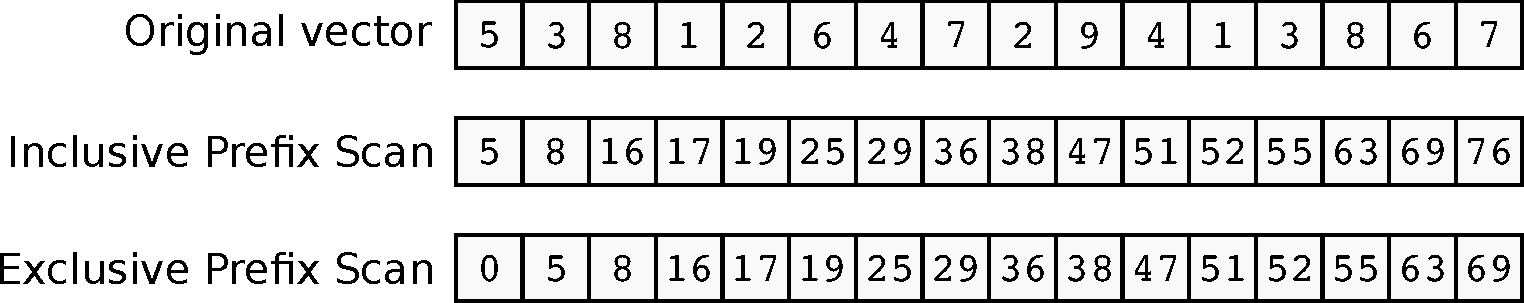
\includegraphics[width=\textwidth]{prefscan_seq}

\vspace{0.3cm}

Both variants are commonly implemented {\it in-place} which mean that
the result is stored in the input array. {\bf The objective of this
exercise is to implement a parallel version of the inclusive prefix
scan using OpenMP}. 

The sequential version of the inclusive prefix scan is extremely
simple and consists of the following lines of code
\begin{verbatim}
  for(i=1; i<l; i++)
    pref[i] = pref[i]+pref[i-1];
\end{verbatim}

As you can see, the above loop cannot be parallelized with a simple
\texttt{\#pragma omp parallel for} directive because of a loop-carried
dependency (iteration \texttt{i} uses the result of iteration
\texttt{i-1}). For this reason a more complicated algorithm has to be
used; this methods consists of the following 5 steps:
\begin{enumerate}
\item the initial vector is split into four chunks (parts) of roughly
  the same size and each chunk is assigned to one thread;
\item each thread computes the inclusive prefix scan of the chunk it
  was assigned;
\item each thread copies the last element of its local result into the
  corresponding location of a temporary array \texttt{loc\_last}
  (i.e., thread number 0 will copy the value in \texttt{loc\_last[0]},
  thread number 1 in \texttt{loc\_last[1]} etc.);
\item {\bf one} thread (it can be the master as well as any other
  thread, but only one) computes the {\bf exclusive} prefix scan of
  the \texttt{loc\_last} array;
\item each thread sums the corresponding element of the resulting
  \texttt{loc\_last} array into its own chunk.
\end{enumerate}

Here is an example of how this algorithm is applied to the vector in
the previous figure when the number of threads is equal to 4:

\vspace{0.3cm}

\noindent\includegraphics[width=\textwidth]{prefscan_par}

\section{Package content}

The \texttt{PrefixScan} directory contains a single file named
\texttt{prefixscan.c}.
This file contains:
\begin{itemize}
\item a sequential inclusive prefix scan routine
  \texttt{prefix\_inc\_seq} that takes two arguments:
  \begin{enumerate}
  \item an integer \texttt{l} containing the length of the array whose
    prefix scan has to be computed;
  \item a reference \texttt{*pref} of the array whose
    prefix scan has to be computed;
  \end{enumerate}
\item a sequential exclusive prefix scan routine
  \texttt{prefix\_exc\_seq} with the same
  interface as the inclusive routine;
\item the declaration of the parallel inclusive prefix scan routine
  \texttt{prefix\_inc\_par} (at the beginning the routine is empty and
  the objective of the exercise is to write it);
\item a main program that creates a vector, fills it with random
  numbers, computes the inclusive prefix scan with both the sequential
  and the parallel version and finally checks that the result of the
  parallel version is the same as that of the sequential one.
\end{itemize}

The code can be compiled with the \texttt{make} command: simply type
\texttt{make} int the \texttt{PrefixScan} directory. This will
generate an executable \texttt{main} file that can be run like this
\begin{verbatim}
$ ./main l
\end{verbatim}
where l is the length of the array whose prefix scan has to be
computed. Obviously, at the beginning the execution of the main
program will report an error because the parallel version is not
implemented.

\section{Assignment}
\begin{itemize}
\item {\huge \Keyboard} Implement the parallel inclusive prefix scan
  algorithm described above using OpenMP inside. Compile and run the code
  with 1, 2 and 4 threads to check the correctness of your parallel
  implementation.
\item \smallpencil Did you observe any speedup (reduction of the
  execution time) when using 2 or 4 threads instead of 1? If not, how can
  you explain this? report your comments in the \texttt{responses.txt}
  file.
\end{itemize}


\paragraph{Advice.}
\begin{itemize}
\item Note that inside the empty initial version of the parallel
  routine, the \texttt{loc\_last} array is already declared of size
  \texttt{MAXTHREADS} (equal to 16). Clearly you only have to use the
  first \texttt{nth} elements where \texttt{nth} is the number of
  threads in your parallel region.
\item Pay attention to the synchronization between threads.
\item Note that the original vector is only logically partitioned into
  chunks: this means threads don't have to allocate memory for storing
  the local chunks but that each thread simply has to identify the
  first element and the length of its own local chunk.
\item Use the \texttt{prefix\_inc\_seq} sequential routine to compute
  the inclusive prefix scan on the local chunks as described in step 2
  of the parallel algorithm. Use the \texttt{prefix\_exc\_seq} routine
  to compute the exclusive prefix scan of the \texttt{loc\_last} array
  as described in step 4 of the parallel algorithm.
\item Compile with \texttt{make main\_dbg} to get some messages useful
  for debugging.
\end{itemize}




\end{document}

%%% Local Variables: 
%%% mode: latex
%%% TeX-master: t
%%% End: 
